% file: C18_domain.tex
% author: C. Menges

\documentclass{standalone}
\usepackage{tikz}
\usetikzlibrary{arrows}
\begin{document}
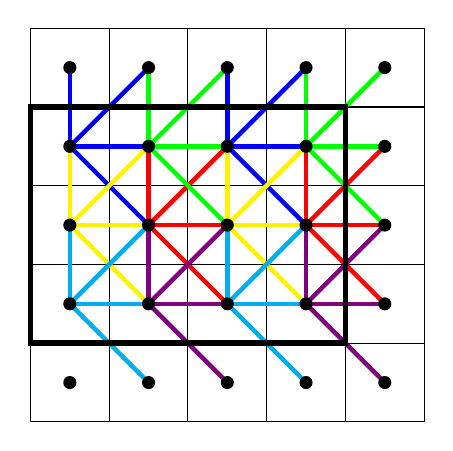
\begin{tikzpicture}

  % grid
  \draw[step=1.0,black,thin,shift={(-2.5,-2.5)}] (0,0) grid (5,5);

  % interactions
  \foreach \col [count=\j, evaluate=\j as \i using {mod(\j,2)+1}, evaluate=\j as \y using {mod(\j,3)-1}] in {red,blue,violet, yellow, green, cyan} {
      \foreach \x in {-3,-1} {
          \draw [ultra thick, \col] (\x+\i,\y) -- (\x+\i+1,\y);
          \draw [ultra thick, \col] (\x+\i,\y) -- (\x+\i,\y+1);
          \draw [ultra thick, \col] (\x+\i,\y) -- (\x+\i+1,\y+1);
          \draw [ultra thick, \col] (\x+\i,\y) -- (\x+\i+1,\y-1);
        }
    }

  \foreach \x in {-2,...,2} {
      \foreach \y in {-2,...,2} {
          \draw[fill=black] (\x,\y) circle (.5ex);
        }
    }

  \draw [line width=2pt] (-2.5,-1.5) rectangle (1.5,1.5);
\end{tikzpicture}
\end{document}